\documentclass[a4paper]{report}
\usepackage{fullpage} % Slightly more margins
\usepackage{fontspec}
\usepackage[usenames,dvipsnames]{color}
\usepackage{fancyhdr}
\usepackage[english]{babel}
\selectlanguage{english}
%\usepackage[utf8]{inputenc} % XeLaTeX doesn't need this
\usepackage{graphicx}
\usepackage{url}
\usepackage[colorlinks=true]{hyperref}
\usepackage{amsmath}
\usepackage{amsfonts}
\usepackage{amssymb}
\usepackage{lastpage}
\usepackage{pgf}
\usepackage{wrapfig}
\usepackage{parskip}
\usepackage{listings} % Source code highlighting
\usepackage{algpseudocode} % Algorithms

\pagestyle{fancy}
% Create header and footer
\headheight 27pt
\pagestyle{fancyplain}
\lhead{}
\chead{}
\rhead{}
\lfoot{}
\cfoot{\thepage}

\addto\captionsenglish{\renewcommand{\chaptername}{Code Sample}}

% Create title page
\title{The Code Challenge 2015}
\author{Mottagningen}
\date{2015-08-18}

\lstset{
				basicstyle=\footnotesize\ttfamily,
				numbers=left,
				frame=l,
				keywordstyle=\color{blue},
                stringstyle=\color{red},
                commentstyle=\color{green},
                identifierstyle=\color{red!50!blue},
                showstringspaces=false,
                extendedchars=true,
                inputencoding=utf8x,
                breaklines=true
}

\begin{document}
\pagenumbering{Roman}
\maketitle
\setcounter{page}{2}

\chapter*{About the Code Challenge}
The Code Challenge is a ``fun-for-the-whole-family'' experience in which you
will try to guess which programming languages are being used to solve a
typical problem which may be solved by code. The forthcoming challenge is an
implementation of a mathematical problem to create a list of prime numbers
up until a certain number. The practical application for such a computer
program might be to find prime numbers that create the basis for a
asymmetrical cryptographic key which is the very foundation for secure
transactions in digital environments.

In front of you lies 21 samples of different programming languages
\footnote{Maybe. Unless we decided to add or remove a few languages.
    In which case there are $n$ language for a $n \in \mathbb{Z}^+$}
where some are well known and some are obscure and really mean.
Your task is to make a qualified guess at which each programming language is.

\newpage
\pagenumbering{arabic}
\setcounter{page}{0}
\chapter{}
\lstinputlisting[language=Java]{../Prime.java}
\chapter{}
\lstinputlisting[language=C]{../prime.c}
\chapter{}
\lstinputlisting[language=Ada]{../prime.adb}
\chapter{}
\lstinputlisting[language=Python]{../prime.py}
\chapter{}
\lstinputlisting[language={}]{../prime.go}
\chapter{}
\lstinputlisting[language=Haskell]{../prime.hs}
\chapter{}
\lstinputlisting[language={}]{../prime.cs}
\chapter{}
\lstinputlisting[language={}]{../prime.lua}
\chapter{}
\lstinputlisting[language=PHP]{../prime.php}
\chapter{}
\lstinputlisting[language={}]{../prime.js}
\chapter{}
\lstinputlisting[language={}]{../prime.vala}
\chapter{}
\lstinputlisting[language={}]{../prime.erl}
\chapter{}
\lstinputlisting[language={}]{../prime.clj}
\chapter{}
\lstinputlisting[language=Cobol]{../prime.cob}
\chapter{}
\lstinputlisting[language={}]{../prime.ps1}
\chapter{}
\lstinputlisting[language={}]{../prime.cpp}
\chapter{}
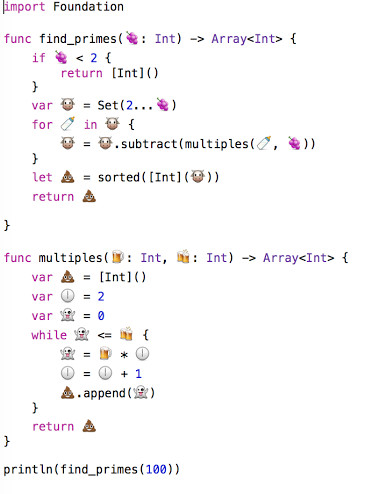
\includegraphics[scale=0.6]{swift}
\chapter{}
\lstinputlisting[language={}]{../prime.vim}
\chapter{}
\lstinputlisting[language={}]{../prime.rs}
\chapter{}
\lstinputlisting[language=Perl]{../prime.pl}
\chapter{}
\lstinputlisting[language=Prolog]{../prime.pro}
\end{document}
